\documentclass{article}

\usepackage{times}
\usepackage{graphicx}
\usepackage[numbers]{natbib}
\usepackage{algorithm}
\usepackage{algorithmic}
\usepackage{hyperref}
\usepackage[accepted]{icml2016}
\usepackage{amsmath}
\usepackage{subcaption}
\usepackage{qtree}
\usepackage{titlesec}
\usepackage{csvsimple}

\begin{document}
\twocolumn[\icmltitle{An Approach to Off-line Handwriting Recognition through Segmentation Techniques and Deep Neural Networks}
\icmlauthor{Jarre Knockaert}{Jarre.Knockaert@UGent.be}
\icmlauthor{Ruben Dedecker}{Ruben.Dedecker@UGent.be}

\vskip 0.3in
]
\begin{abstract}
The aim of this paper is to present a complete system for off-line handwriting recognition.
We discuss how to segment handwritten text through contouring. Next we present our method of segmenting words into characters.
Then we propose a method to recognize characters with a deep neural network.
Finally we present postprocessing techniques to correct mispredicted text.
Our approach does not outperform state-of-the-art systems but hopes to provide a thorough elaboration for every step in the process.
\end{abstract}

\section{Introduction}
Despite the expontially increasing amount of digital information in the contemporary world, a lot of new documents are still handwritten.
Handwritten documents are very inefficient as they need to be read manually in order to extract information.
These documents need manual labour and physical space in order to be stored in an organized manner.
Finally, it takes a lot of time, effort and resources to move these documents to another location.

This paper presents an off-line handwriting recognition system. This system digitizes handwritten texts, which allows modern data processing, storage and transmission techniques to be applied to the information stored in the handwritten documents.
We only cover off-line handwriting recognition in this paper, where we have the full handwritten text in advance. This problem is similar to Optical Character recognition (OCR). OCR digitizes printed texts, this is generally easier to recognise as it contains less variation than handwritten texts.
On-line recognition on the other hand converts text as it is written (on a touchscreen for example). Other information is available for this problem, e.g. the exact movements of the pen. \cite{olcr} present a technology for online recognition of Japanese handwritten text with an accuracy of 94.6\%.

First we explain how to recognise characters in Section \ref{sec:charrec}. This explanation involves the used dataset, preprocessing techniques and the deep neural network for classifying characters.
In Section \ref{sec:segtext} we describe how to segment a text into words using a contouring algorithm with consequent postprocessing to remove unwanted noise.
After this we present our approach to seperating the characters from words in \ref{sec:segword}. We use vertical projections combined with postprocessing techniques including a neural network for segmentation point evaluation.
Postprocessing steps are presented in Section \ref{sec:postproc}, we try to correct word recognition errors using an English dictionary and language models, n-gram models in particular.
We conclude this paper with some experimental results, the problems we encountered combined with possible improvements. A complete flow of the recognition of an image is shown in Figure \ref{fig:flow}.

\begin{figure*}
  \centering
  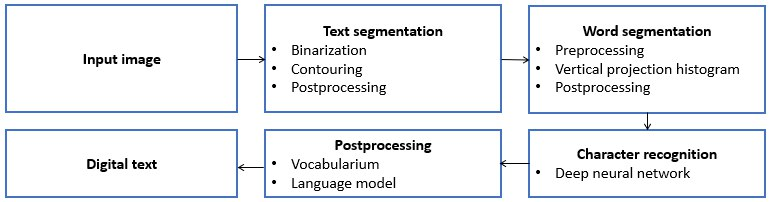
\includegraphics[width=\linewidth]{images/flow_hor}
  \caption{All of the steps in our system to convert an image with handwritten text to digitalized text.}
  \label{fig:flow}
\end{figure*}

\section{Character Recognition}
\label{sec:charrec}
The smallest distinguishable token in a text is a character. These handwritten characters are uniquely
written by each individual and variations even occur when written by the same individual. These variations include the inclination of characters (i.e. the slant) orientation and size.
A way of dealing with these includes removing variations from the input image using preprocessing techniques.
We take another approach, instead of adding rules to minimize variations we made a deep neural net which can recognise any character with a certain probability. The architecture of this deep neural network is described in Section \ref{sec:dnn}.
In order to make the deep neural network recognize characters in images with these variations, we augmented the dataset to include a bigger variety of images. We present these augmentation techniques in Section \ref{sec:preproc}.
The dataset of handwritten characters is described in Section \ref{sec:data}.

\subsection{Dataset}
\label{sec:data}
Before exposing the neural network to new characters, it needs to be familiar with many training samples to be able to classify any new character correctly.
This is why a good dataset is very important. A dataset should have many examples, much variation, and an even balance between classes. A dataset with these properties
allows the neural network to train effectively and recognize any new character given to the network.

We use the Chars74K dataset for this purpose. It has 3410 images with handwritten characters, each belonging to one of 62 classes (0-9, A-Z, a-z).
This dataset contains both very easily recognisable images of characters but also characters which are even hard to recognise for humans, as shown in Figure \ref{fig:char}.
3410 input images is quite low for a neural network to be effectively trained. To overcome this problem we employ some data augmentation techniques discussed in Section \ref{par:aug}.

\begin{figure}
\begin{subfigure}{.23\textwidth}
  \centering
  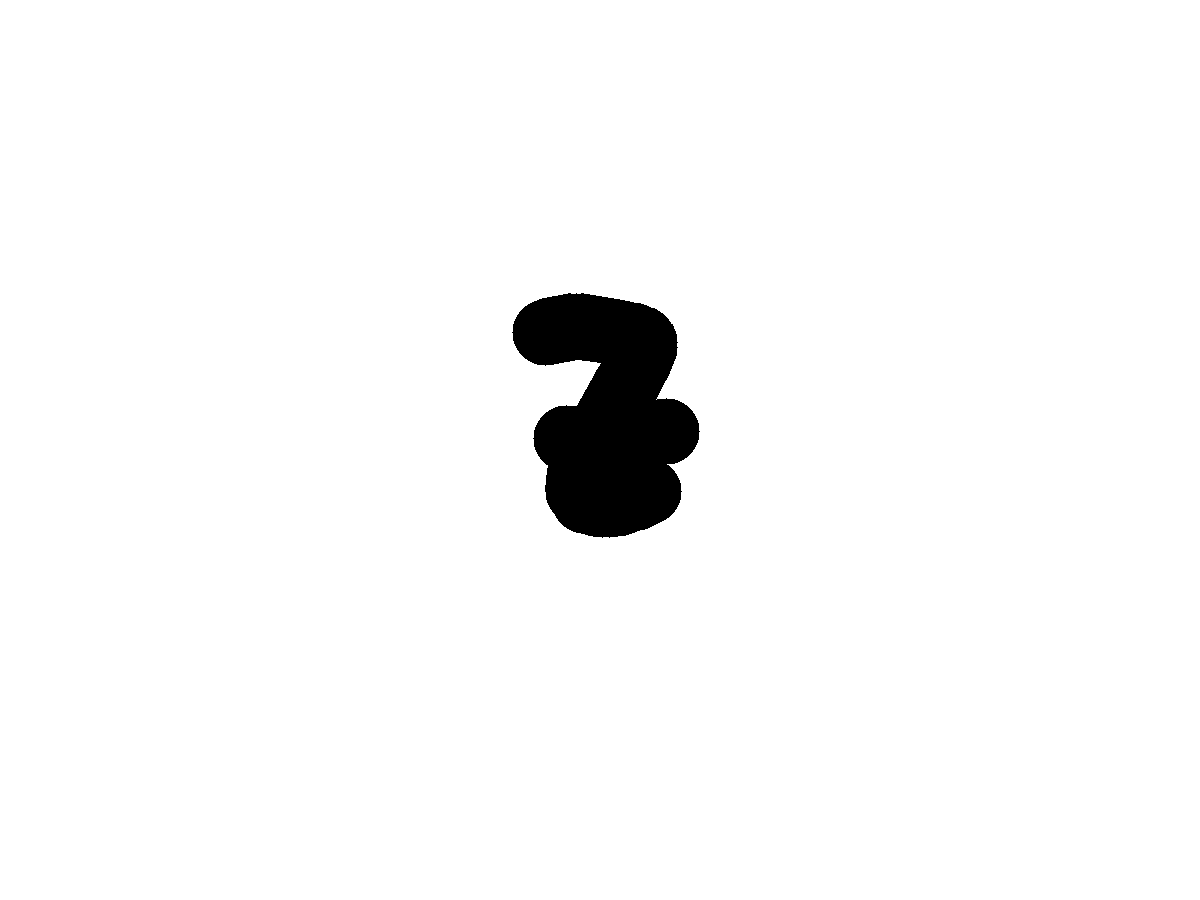
\includegraphics[height=2cm]{images/bad_char1}
\end{subfigure}
\begin{subfigure}{.23\textwidth}
  \centering
  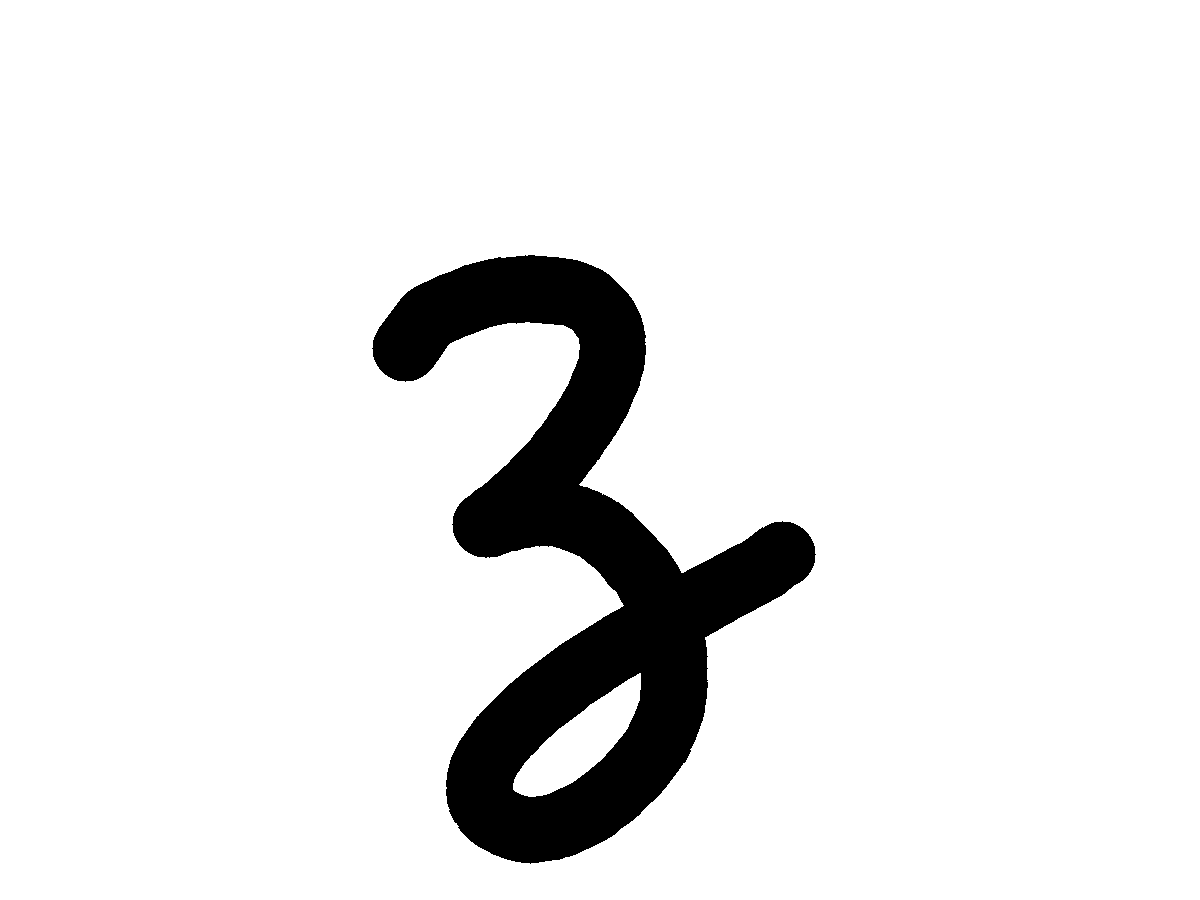
\includegraphics[height=2cm]{images/bad_char2}
\end{subfigure}
\caption{Examples of written 'z' characters, which are hard to recognise or are ambiguous.}
\label{fig:char}
\end{figure}


\subsection{Preliminary steps}
\label{sec:preproc}
We make use of two types of preprocessing steps: normalization and augmentation of the data. Normalization of data adjusts the original data and data augmentation takes the data and uses augmentation techniques to create variations of the original data.

\subsubsection{Normalizing data}
\label{par:norm}
Theoretically feeding normalized data to the neural network returns the same output as before.
In reality however, it is better to normalize data to avoid getting stuck in local optima and to increase training speed of the model \cite{NormGoal}.
We normalize the data by reducing the input dimensions to (64,64,1). A simple threshold is added to improve the contrast in our image.
This allows the foreground to be more distinguishable from the background and allows the neural network to train and recognize characters more easily.

\subsubsection{Data augmentation}
\label{par:aug}
Data augmentation serves two purposes. It makes the dataset more robust to different kinds of handwriting as we add variations of the original data to the training samples.
The second purpose is to increase the size of our dataset. As our dataset only contains 3410 images of handwritten characters, we need more data for the neural network to be able to function properly.
Next we will describe the data augmentation techniques we used. For these techniques we based us on \cite{DataAug}. A more thorough explanation can be found there.

\paragraph{Translations of data}
The dataset is extended with variations in padding of characters in images. For this purpose we multiply every coordinate of the original image with the following transformation matrix:
\begin{equation}
        \begin{bmatrix}
                1 & 0 & t_x \\
                0 & 1 & t_y
        \end{bmatrix}
\end{equation}
where $t_x$ is the horizontal shift and $t_y$ is the vertical shift. The values for chosen for $t_x$ are -16, 0 and 16, the values chosen for $t_y$ are -8, 0 and 8. All combinations are used except $t_x=0$ and $t_y=0$. The translation only occurs if it does not move the character outside of the image.
\paragraph{Rotations of data}
Rotations of the image are added to the dataset to make the network more robust to handwritings with different orientations. The transformation matrix is equal to:
\begin{equation}
       \begin{bmatrix}
               \alpha & \beta & (1-\alpha)*center.x - \beta*center.y \\
               -\beta & \alpha & \beta*center.x + (1-\alpha)*center.y
       \end{bmatrix}
\end{equation}
where $\alpha = cos(angle)$ and $\beta = sin(angle)$. $center$ is the coordinate in our image around which is rotated and the angle describes the amount of degrees to rotate in the clockwise direction. We use -30 and 30 as angle.
\paragraph{Scaling of data}
With the purpose of making the network more robust to different sizes of handwriting, we add different scalings of the data. We scale in both the horizontal and vertical direction. The following transformation matrix allows us to scale the input image:
\begin{equation}
       \begin{bmatrix}
               s_x & 0 & 0  \\
               0 & s_y & 0
       \end{bmatrix}
\end{equation}
where $s_x$ is the horizontal scaling factor and $s_y$ is the vertical scaling factor.
We use combinations of values in $[0.75, 1, 1.25, 1.5]$ for $s_x$ and $s_y$ depending on the original size of the character.
\paragraph{Shearing of data}
In order to deal with different kinds of slants we add sheared versions of the image to the dataset.
Shearing displaces each point in a fixed direction, by an amount proportional to its signed distance from a line that is parallel to that direction \cite{Shear}. We used the following shear mapping to achieve this:
\begin{equation}
        \begin{bmatrix}
                1 & s & 0 \\
                0 & 1 & 0
        \end{bmatrix}
\end{equation}
\paragraph{Erosion of data}
The erosion operation of images adds thinner versions of characters to the dataset. Erosion uses a kernel to convolute an image.
The image is scanned using the kernel. The maximum pixel value of the overlapping part between the image and the kernel is computed. This pixel value of the anchor point of the kernel is replaced with the maximum pixel value.
This causes bright regions to get thinner and dark regions to get bigger in the image.

All of the previously discussed preprocessing techniques are also applied to the eroded image. The final dataset contains translated, orientated, sheared and scaled versions of both the original image and the eroded image. A visualitation of the augmentation of a picture can be seen in Figure \ref{fig:augmented}.

\begin{figure}
\begin{subfigure}{0.15\textwidth}
  \centering
  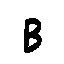
\includegraphics[width=\linewidth]{images/original}
  \caption{Original}
\end{subfigure}
\begin{subfigure}{0.15\textwidth}
  \centering
  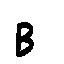
\includegraphics[width=\linewidth]{images/translated}
  \caption{Translated}
\end{subfigure}
\begin{subfigure}{0.15\textwidth}
  \centering
  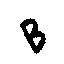
\includegraphics[width=\linewidth]{images/rotated}
  \caption{Rotated}
\end{subfigure}
\begin{subfigure}{0.15\textwidth}
  \centering
  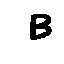
\includegraphics[width=\linewidth]{images/scaled}
  \caption{Scaled}
\end{subfigure}
\begin{subfigure}{0.15\textwidth}
  \centering
  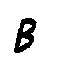
\includegraphics[width=\linewidth]{images/sheared}
  \caption{Sheared}
\end{subfigure}
\begin{subfigure}{0.15\textwidth}
  \centering
  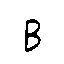
\includegraphics[width=\linewidth]{images/eroded}
  \caption{Eroded}
\end{subfigure}
\caption{An image transformed by the discussed augmentation techniques.}
\label{fig:augmented}
\end{figure}
\subsection{Deep neural network}
\label{sec:dnn}
Humans have millions of connected neurons in the visual cortices which are capable of image processing.
We can recognize most characters without any thought because of this complex neural network inside our brain.
For computers, character recognition is a more difficult task. We could try to write rule-based systems and define how every character should look. This solution is not flexible at all and is very hard to define.
We use a neural network, inspired by how the brain processes images. These deep neural networks contain several layers of connected perceptrons, where each connection is defined by a weight and each perceptron is defined by a bias.
The perceptrons take an input and calculate an output using an activation function. This allows perceptrons to make decisions.
Normalized images can be fed to the neural network, which then propagate through several layers and eventually produce as output the probability that the input image has a certain class, one of the possible characters.
Now follows a detailed overview of our deep neural network. This overview is visualized in Figure \ref{fig:dnn}. A detailed explanation on how deep neural networks function is explained by \cite{nnbook}.

\begin{figure*}
  \centering
  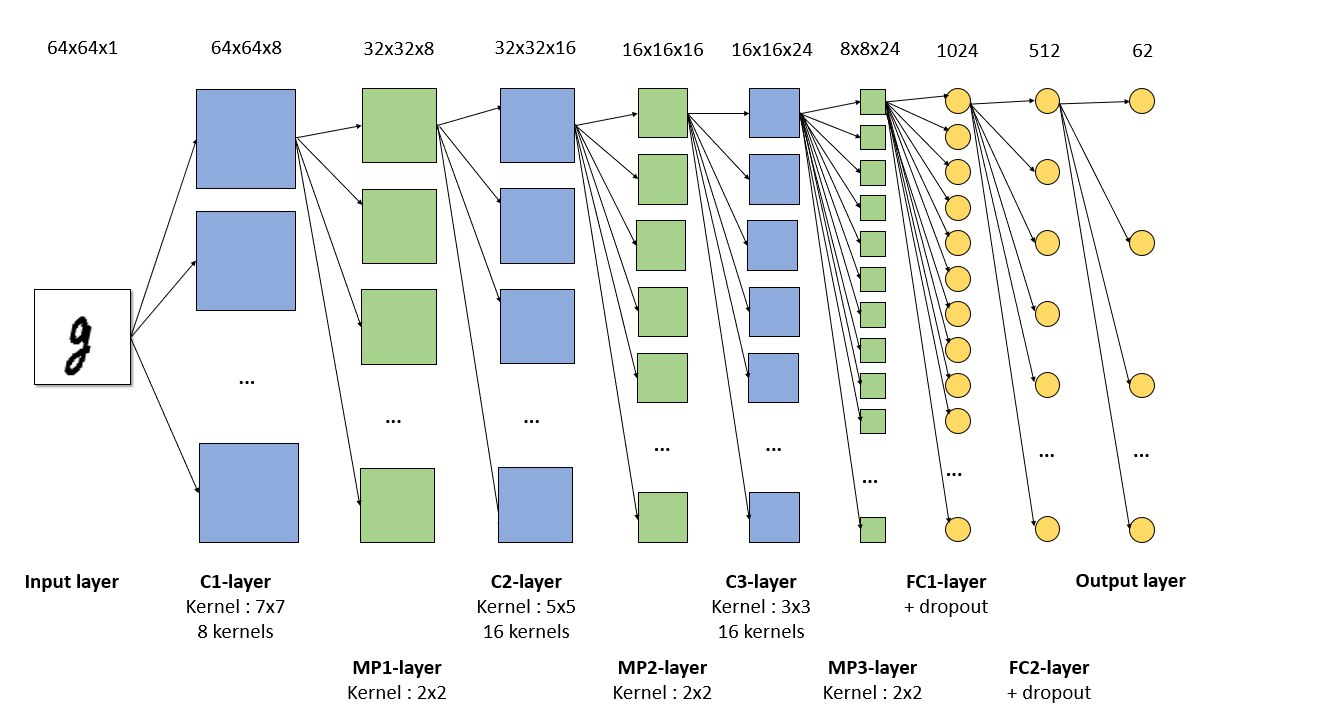
\includegraphics[width=\textwidth]{images/dnn}
  \caption{Visualization of the deep neural network for character recognition. The first row shows the shape of a layer. The second row shows the visualization of that layer, the third row shows information about the layer. 'C' indicates a convolutional layer, 'MP' a max-pooling layer and 'FC' a fully-connected layer.}
  \label{fig:dnn}
\end{figure*}

\subsubsection{Convolutional layers}
 The input is a normalized image with one color channel. This is fed to a convolutional layer. Convolutional layers allow us to extract features by scanning the image with filters. These features might be edges, corners or any other type of shape in the image. The extracted features are called a feature map.
 We can apply several of those filters using one convolutional layer to extract several types of features.
 This works because images have a spatial structure; i.e. close pixels have shared information. By applying a filter, pixels in the same region will use shared biases and weights, which allows the filter to extract particular features.
 Next we add a pooling layer, in particular a max-pooling layer. Pooling layers remove the positional information of the features in the image. This is useful because the exact location is less important than the location relative to the other features and this allows us to reduce the amount of parameters required in the next layers.
We use three convolutional layers combined with max pooling layers in order to extract low, medium and high level features.
\subsubsection{Fully-connected layers}
Next we flatten the output of the last convolutional layer in order to extract a one-dimensional array from the three-dimensional feature maps. This one-dimensional array can now be fed to a fully-connected layer, which is a layer of connected perceptrons as previously discussed.
There are three fully-connected layers of which the first two are connected with a dropout layer and the last one is the output layer.
Dropout randomly drops units and their connections from the network during training. Dropout greatly reduces overfitting in the fully connected layers. \cite{dropout} We do not use this after the convolutional layers as they are very resistant to overfitting \cite{nnbook}.
The last fully connected layer has 62 output neurons, which correspond to the 62 possible output classes. We use rectified linear units in order to compute the activation function. A rectified linear unit or rectified linear neuron is a unit which uses a rectifier as linear unit. It's output is given by
\begin{equation}
        max(0, w*x+b)
\end{equation}
where $x$ is the input, $w$ is the weight vector and $b$ is the bias.
\subsubsection{Softmax layer}
 The last layer in the neural network is a softmax layer with a cross-entropy cost function. The softmax layer computes a probability distribution (i.e. a set of 62 numbers which sum up to 1) using the 62 output neurons from the previous layer. An element in the probability distribution estimates the probability of the input image to classify as a certain character.
 The cross-entropy cost function uses the actual labels to calculate the error between the actual labels and the predicted labels (the previously discussed probabilities). The closer the cross-entropy value is to zero, the better the neural network is at classifying handwritten characters.
 \subsubsection{Weight adjustment}
Finally, in order to actually train the neural network, we need some kind of weight adjustment. This will effectively improve the decision making of perceptrons and thus, the classification of images.
The Adam optimizer effectively fulfills this goal. In order to explain the Adam optimizer, a few other methods have to be known, a very brief explanation of these methods follow.
First of all, stochastic gradient descent (SGD) is an iterative method that tries to find minima. This function takes a step size which is known as the learning rate. SGD can be used to minimize the cross-entropy function iteratively by adjusting the weights.
Momentum-based gradient descent makes the correction dependent based on an average of several previous corrections to move more quickly in the correct direction.
AdaGrad allows the learning rate to adapt based on parameters. AdaDelta solves a problem of AdaGrad, concerning the learning rate to become so small that learning becomes impossible.
Each of these methods effectively improve the previously mentionned method.
The Adam optimizer, introduced by \cite{adam}, is an optimization of AdaDelta, which uses a distinct learning rate and momentum for every parameter. This optimizer achieves the highest accuracy in our case and will be used.

The Adam optimizer minimizes the error calculated by the cross-entropy cost function adjusted with a weight decay factor. Weight decay regulizes the neural network by penalizing big weights and promoting smaller weights. Neural networks with this constraint tend to overfit less because small weights are less sensible to small changes of the input. \cite{presham}

\section{Segmentation of text into words}
\label{sec:segtext}
In this section we explain the first step in the process of extracting individual characters from a text image: i.e. word extraction.
Word extraction from text images has many possible approaches, but in this paper we focus solely on the word contouring approach, pointed out by following paper \cite{WordSegm} to be a successful word extraction method.
With this method we extract the contours of the words in a given text image. Through postprocessing techniques we can rearrange these extracted words into lines.
The proposed approach focusses solely on text images, and does not take into account non-textual areas found in the input image.
Additional techniques for page segmentation can be utilized depending on the situation.

\subsection{Binarization}
We start with binarizing the text image. To achieve this there are a lot of thresholding algorithms to choose from, but the one we use is a combination of Gaussian blur in combination with Otsu's thresholding algorithm. \cite{Otsu79} 
The Gaussian blur will smoothen the noise in the image and smoothen the edges of the text.
Otsu's tresholding algorithm will deliver adequate result for noisy text documents.
The choise of tresholding algorithm depends mostly on the intended purposes of the algorithm.
Additional noise removal techniques and other preprocessing techniques may be required for a better result when processing images with much noise. 


\subsection{Contouring}
Our text segmentation approach is based on finding contours in the text image.
We can find these contours using the algorithm \cite{Suzuki85}.
Through postprocessing we can recover the original words from these extracted contours.

\subsection{Postprocessing}
We remove the incorrect contours generated by the contouring algorithm through postprocessing.
Next we reconnect words that are split because they are not written in a single stroke.

\subsubsection{Contour removal}
The contouring algorithm can create incorrect contours because of left-over noise in the image.
The tool we will use to remove these contours is a bounding box drawn around the contour.
This bounding box is the smallest rectangle containing the contour, it allows us to easily compare positions of contours in the text image.

Firstly we remove the contours of which the bounding box is inside the box of another contour.
This is possible as text segmentation returns the word in the image contained by its biggest bounding box. 
Secondly we remove contours that are too small to contain possible word parts. These contours consist of noise and punctuation.
These contours are neglected by taking the average height of all the found contours in the text.
We remove all of the contours with a height smaller than $average height * (2/3)$.


\begin{algorithm}[tb]
    \caption{Contour combination algorithm}
    \label{alg:overlap}
\begin{algorithmic}
    \STATE {\bfseries Input:} $contour1$, $contour2$
    \STATE $xGap$ = calculateXaxisDistance $contour1$ $contour2$
    \STATE $yOverlap$ = calculateYoverlap $contour1$ $contour2$
    %TODO ::\IF {$xGap < averageWordWidth * (1 / (averageCharacterCount * 2)) $ {\bfseries and} $yOverlap > min(word1.height, word2.height) * requiredYaxisOverlap$}
    \STATE combineContours $contour1$ $contour2$
\end{algorithmic}
The chosen paramters are:
\\
$averageCharacterCount = 8$ 
\\
$requiredYaxisOverlap = 1/2$
\end{algorithm}

\subsubsection{Contour combination}
The leftover contours are used to to reconstruct the original words from the text.
This is done by combining multiple contours which consist of parts of words belonging to the same word. 
We have created an algorithm \ref{alg:overlap} that decides when to combine two word segments into a single word. 



\begin{algorithm}[tb]
   \caption{Algorithm for line reconstruction}
   \label{alg:linereconstr}
\begin{algorithmic}
   \STATE {\bfseries Input:} $extractedWords$, $textlines$
   \REPEAT
        \STATE $highestWord = findHighestWord $
        \STATE $newline = [highestWord]$
        \STATE Initialize $noChange = true$.
        \STATE $avgY= newline$.findAverageYpos
        \REPEAT
            \FOR{$word$ {\bfseries in} $extractedWords$}
            \STATE $boundRect = word.contour.boundingRect$
            \IF{ $avgY > word.y$ {\bfseries and} $avgY < word.y + word.h$ }
            \STATE $line$.add $word$
            \STATE $noChange = false$
            \ENDIF
        \ENDFOR
        \UNTIL{$noChange = true$}
        \STATE $textlines$.add $newline$
   \UNTIL{$words$.empty $= true$}
\end{algorithmic}
\end{algorithm}

\subsection{Line selection}
As the ordening of the words % TODO, verklaar waarom die ordening weggat? 
we place the words in lines, and orden these lines. 
Algorithm \ref{alg:linereconstr} shows the pseudocode of our line selection process.
The algorithm reorders the words in lines and orders these lines as ordered in the original text.

\begin{figure}
    \begin{subfigure}{\linewidth}
    \centering
    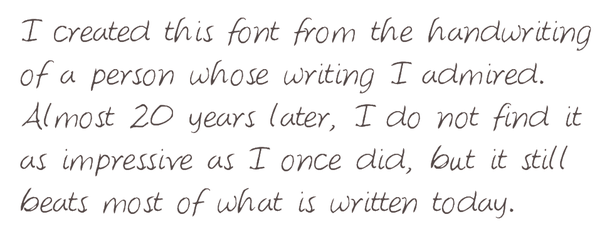
\includegraphics[width=.7\linewidth]{images/text}
    \vspace{-5px}
    \caption*{Original text image.}
    \end{subfigure}
    \begin{subfigure}{\linewidth}
    \centering
    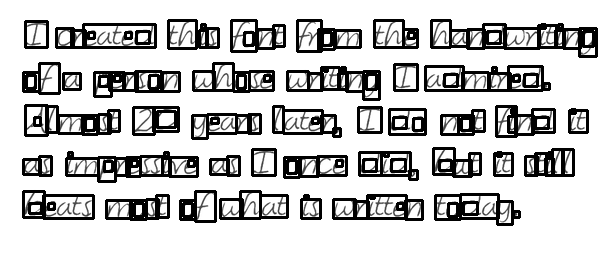
\includegraphics[width=.7\linewidth]{images/cont}
    \vspace{-5px}
    \caption*{Contouring algorithm.}
    \end{subfigure}
    \begin{subfigure}{\linewidth}
    \centering
    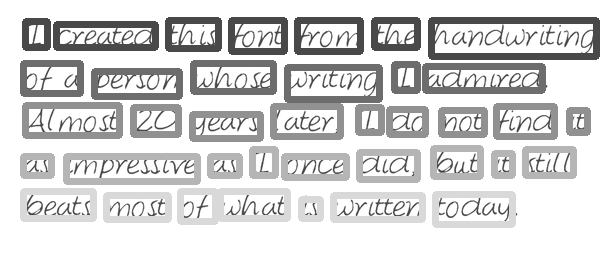
\includegraphics[width=.7\linewidth]{images/lines}
    \vspace{-5px}
    \caption*{Postprocessing and line selection.}
    \end{subfigure}
    \vspace{-10px}
    \caption{Text segmentation steps}
    \label{fig:text_segm}
    \vspace{-20px}
\end{figure}


\section{Segmentation of words into characters}
\label{sec:segword}

The next step in the process is to extract the character images from the found word images.
Again, there is a choice between several different approaches.
In this paper we focus solely on a word oversegmentation approach to character extraction, through skeletonization and using a vertical projection profile. The reasoning begind this can be found in the following papers \cite{CharSegm} and \cite{CharSegmOld}.

After first oversegmenting the word, we will recover the original character through postprocessing steps combining different word segments.

\subsection{Normalization}
The first action is again normalizing the word image.
We will resuze the image to a fixed height of $100px$.
This will result in more consistency in rule-based post processing steps.

\subsection{Binarization}
The word image is binarized.
This is again done with a combination of Gaussian blur and Otsu's method.
The binarization is needed for the next step, because we can only apply a skeletonization algorithm to a binary image.


\subsection{Skeletonization}
Now we will skeletonize our word image.
This will normalize the thickness of the strokes to a single pixel.
This allows us to execute our Verical projection profile and interpret the results easily.
The skeletonization algorithm used is the scipy adaptation of the Zhang Suen thinning algorithm \cite{zsthinning}.

\subsection{Vertical projection histogram}
Using the skeletonized word image, we now create a vertical projection histogram.
This vertical projection histogram takes the sum of every collumn in the image, counting black pixels as a $1$ value, and white pixels as a $0$ value.

We now regard the collumns with a total pixel count of zero or one pixel as potential segmentation points.
We interpret these collumn to be the whitespace in between characters or the line connecting two characters to each other.
This will inevitably cause oversegmentation in our word image.
The next step will be to filter the potential segmentation points, and remove the incorrect ones through postprocessing.

\begin{figure*}
    \begin{subfigure}{0.33\textwidth}
    \centering
    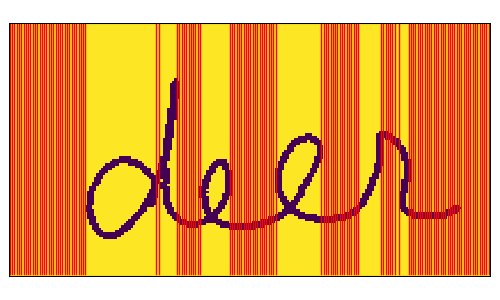
\includegraphics[width=\textwidth]{images/vpp}
    \caption*{Vertical projection profile.}
    \end{subfigure}
    \begin{subfigure}{0.33\textwidth}
    \centering
    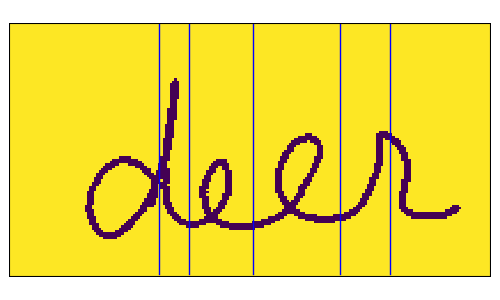
\includegraphics[width=\textwidth]{images/rules}
    \caption*{Rule based correction.}
    \end{subfigure}
    \begin{subfigure}{0.33\textwidth}
    \centering
    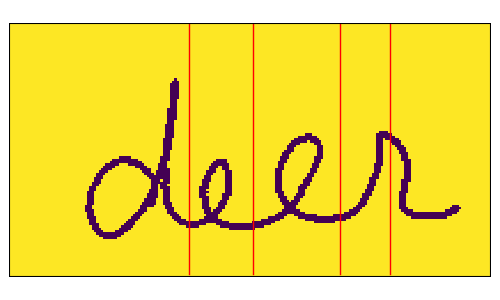
\includegraphics[width=\textwidth]{images/nn}
    \caption*{Correction through neural network.}
    \end{subfigure}
    \caption{Word segmentation steps}
    \label{fig:char_segm}
\end{figure*}

\subsection{Oversegmentation correction}
In this section we provide techniques to verify the correctness of segmentation points.
\cite{evalsplitpoints} discusses three approaches to evaluate segmentation point correctness: rule based techniques, cost function optimization based methods and machine learning based procedures.
In this paper we discuss machine learning based approaches precedented by a few rule based techniques.

\subsubsection{Rule based techniques}
The main oversegmentation correction is handled by our neural network.
However some simple preprocessing is added to remove obvious unwanted segmentation points.

We first remove removes the segmentation points found at the start and the end of the word image.
These segmentation points are an artifact of the used segmentation approach, as can be observed in Figure Figure \ref{fig:char_segm}.
These points can be removed without information loss, as the alphabet does not contain letters that entirely convert to a single pixel line after skeletonization.

Subsequently we group consequent segmentation points.
The occurence of these consequent segmentation points is another artifact from our segmentation approach, as can be seen in Figure \ref{fig:char_segm}.

From these groups of points, we take the center point as the new potential segmentation points.
However if one or more of the segmentation points in the group stems from empty collumns, the new segmentation point is chosen as the center point of the points representing the empty collumns in the word image.

Finally we aggregate groups of consequent potential segmentation points, separated by collumns containing less pixels than a certain threshold value $maxSumThresh$.
We have chosen a conservative value of $3px$ for this threshold.
This remedies the segmentation of slated lines inside characters, which can be an artifact of the skeletonization algirithm used.

A technique was tested using the feedback of the chracter recognition network to remove incorrect segmentation points.
However this turned out not to be ineffective, because the neural network tends to provide random probabilities with a high degree of certainty when images of multiple characters together were fed to the nerual network.
Since it is impossible to validate these responses from the neural network, this approach was abandoned and is not used in the final version.

More rule based filter could be added for more optimal processing of the potential segmentation points.
However the focus of our segmentation correction is the neural network used to remove incorrect segmenatation points.


\subsubsection{Machine learning approach}
The neural network we use to judge the correctness of segmentation points, is based on \cite{evalsplitpointsnn}. The paper explains how to use neural networks to classify the correctness of segmentation points. The discussed algorithm is as follows. Manual classification of segmentation points creates training data with two classes, correct and incorrect segmentation points.
For every of these segmentation points a pixel matrix is extracted surrounding the segmentation point. This pixel matrix is normalised in size.
Next, small windows of equal size are extracted from the pixel matrix and for each window the density is calculated. This is the number of black pixels divided by the total amount of pixels in the window.
With every matrix a corresponding label is encoded for storage in the training file, this label is encoded as 0.9 if the segmentation point is correct and 0.1 otherwise. Now these matrices and corresponding labels are used to train the neural network.

We take a slightly different approach and consider a deep neural network to tackle this problem. This allows us to use the power of convolutational layers to extract features, instead of manually creating features (features which show the density in this case).
We use one convolutional layer and three fully connected layers in our neural network. This neural network takes the actual image of the segmentation point as input (a pixel matrix of the pixels surrounding the splitting point) and returns a one-hot encoded vector indicating if the splitting is correct or incorrect. In order to create training data we created a small program to iterate over splitting points of handwritten words from the IAM dataset. \cite{iam}

This method allowed us to achieve an accuracy of 72 \%, which is still fairly low because of the difficulty of the problem and the small amount of traing data. However this is better than our accuracy with an implementation of the method described by \cite{evalsplitpointsnn}.
Segmentation points can now be filtered if the neural network decides a segmentation point is incorrect.

\subsection{Normalization}
The character normalization step consists of two parts.
Firstly the character is padded untill the height equals the width.
A precondition for the padding step is that the image is already binarized, so that we can use white borders as padding, and this will not distort the image should binarization take place in a later stage.
The image is then resized to $44px x 44px$
Secondly padding of $10px$ is added on all sides of the character image to create whitespace around the letter.
We end up with a $64px x 64px$ character image.
The extra $10px$ padding is to make sure the letters do not stick to the edges, since the Chars74K dataset we work with utilizes borders around the provided characters. Should these borders be removed in the training process however, this should be reflected in this step by ignoring this new padding.

\section{Natural language processing}
\label{sec:postproc}

To cope with some of the errors from the previous steps, there needs to be some kind of correction. This correction should allow the system to reproduce possible written text even when a step of the larger system fails.
In order to do this we adapt natural language processing techniques as postprocessing steps. Natural language techniques can often be found in speech recognition, language generation and other systems.
As a first step we match words against a dictionary to find out if they are syntactically correct, this is discussed in Section \ref{sec:voc}. The second step checks if those given words make sense in the context, this is discussed in Section \ref{sec:lm}.

\subsection{Vocabularium}
\label{sec:voc}
The neural network does not only produce which character is recognised, but rather a list of probabilities indicating the likelihood of an image to be a certain character. We can use all of this information in this postprocessing step instead of throwing that information away and naively returning the most likely character as the actual character.
\begin{figure}
        \Tree [.{(Y, 0.9)}
        [.{(Ye , 0.72)} {(Yes, 0.432)} {(Ye5 , 0.288)} ]
        [.{(Yl , 0.18)} {(Yls, 0.108)} {(Yl5 , 0.072)} ]
            ]
\caption{The first element of a possible list of trees for the word 'Yes' with branching factor 2. The characters have the following probabilities: $P(Y)=0.9, P(T)=0.1, P(e)=0.8, P(l)=0.2, P(s)=0.6, P(5)=0.4$. Other characters have probabilities which are neglible.}
\label{fig:wordtree}
\end{figure}
We make a tree, as shown in Figure \ref{fig:wordtree}, where every node is a tuple with a word (sequence of characters) and a probability (likeliness of that word based on the probabilities of individual characters). The probability is calculated as the product of probability for each character: $P(c_1, c_2,...,c_k) = \prod\limits_{i}{c_i}$ with $1 \leq i \leq k$. In order to keep the complexity low we only consider the three most probable characters. This will be the branching factor of every tree. A tree exists for every possible starting character.
Now we have a list of possible words and their probabilities (every leaf). The closest matches in the dictionary for each word are calculated using the function \textbf{get\_close\_matches} from the python library difflib. \textbf{get\_close\_matches} finds close matches in the English dictionary and their corresponding score.
We multiply this score with our previously calculated probability. This leaves us with a list of correct English words and a score for every word. If we only want to convert the image of one word into text, we can just return the word with the highest score.
This finalises the logic for recognising handwritten words. Next we will discuss a postprocessing technique which is useful when the word is part of a bigger context.
\subsection{Language model}
\label{sec:lm}
Besides checking the syntax of words, we can also look at the context. This is were language models are useful. We can check the previous words and calculate the likeliness of a word to be the next word in the context. N-gram models are used to calculate probabilities given $n-1$ previous words. The probability is computed as $P(w_i | w_{i-n},...,w_{i-1})$.
We use the Markov assumption here: the probability of a word in the context can be approximated by the previous $n-1$ words. \cite{markov} This probability is calculated as follows:
\begin{equation}
        P(w_i | w_{i-n},...,w_{i-1}) = \frac{count(w_{i-n},...,w_{i-1},w_{i})}{count(w_{i-n},...,w_i)}
\end{equation}
where $w_i$ is the word of which we want to calculate the probability and $count(w_i,...w_{i+n})$ indicates the amount of occurences of $w_i,...,w_{i+n}$. That amount is the same as counting the amount of n-grams with that sequence of words. An n-gram is a sequence of n words from a given sequence of text, denoted as $w_i,...,w_{i+n}$. \cite{ngrams}
We use the n-grams from the Google dataset for this purpose. \cite{google} Querying these datasets locally takes several minutes and this happens for every word. Instead we use a Python library phrasefinder to make online queries to these corpora. This greatly increases speed but has the disadvantage of requiring internet connection.
Now we can make queries such as "I like dogs / cats / sheep". Using the Google corpora probabilities are calculated with n-gram models for each of the three words. This gives us a probability for every word based on the context.
Combining the results with the probabilities calculated in Section \ref{sec:voc}, we can
calculate a new score. The word with the highest score is accepted as written word.
The concludes our full system of recognising handwritten texts. In the next section we will further discuss the results of these techniques and some experiments to check the performance and impact of optimizations.
\section{Experimental results}
\label{sec:expres}

\subsection{Character Recognition}
The deep neural network can recognise characters with an accuracy of 91 \%. This neural network was trained for 1000 iterations which took 8650 seconds. We used a learning rate of $10^{-4}$, 256 as batch size, dropout layers with a keep probability of 0.5 and $10^{-3}$ as weight decay. Experimental findings led us to these values.

Comparisons are hard to find as few papers discuss off-line handwritten character recognition.
One paper we found, \cite{charrec}, achieves an accuracy of 98.5 \%, they classify 38 classes (10 digits, 26 letters, 2 special symbols) and manually extract features for the neural network instead of using convolutional layers.

\subsection{Influence of data augmentation on character recognition}

We're using the following setup for this experiment. Every experiment uses the original data in addition with the augmented data using one particular preprocessing technique. The base case without preprocessing techniques, just uses a copy of every image as augmented dataset.

In order to limit the time these experiments run we added some small constraints. We only run every experiment 200 epochs, running these experiments longer might result in different conclusions.
Next it is important to note that a lot of stochastic behaviour is part of these neural networks because of the dropout layers. We run every configuration four times. Only the result with the highest accuracy is considered to avoid outliers.
The accuracy decreases when using preprocessing techniques because the variety of our dataset increases but these techniques allow a more robust neural network which can recognise characters which includes images with more variation.

Table \ref{tab:preprocess} shows that augmentation techniques have great influence on the performance of the neural network. However these results might seem counterintuitive.
All preprocessing techniques have a lower accuracy than the base case. The amount of decrease in accuracy can be explained by how much the original image and the augmented image differ. The configuration with erosion achieves the second highest accuracy, as these images resemble the original images, the shape, position and rotation of the image remains, only the density of regions in the image has changed. A dataset with rotated images instead has much lower accuracy. As the input pixel matrix is completely different, the pixels are in other positions and the original shape has changed.

\begin{table}
\caption{Influence of augmentation techniques on performance of the neural network.}
\label{tab:preprocess}
\vskip 0.15in
\begin{center}
\begin{small}
\begin{sc}
\begin{tabular}{lcc}
\hline
\abovespace\belowspace
Configuration & Accuracy (\%) & Time (s) \\
\hline
\abovespace
No preprocessing & 88.52 & 236 \\
Erosion & 80.95 & 410 \\
Scaling & 66.10 & 271 \\
Rotation & 64.47 & 228 \\
Shearing & 74.36 & 367 \\
Translation & 70.47 & 306 \\
\hline
\end{tabular}
\end{sc}
\end{small}
\end{center}
\vskip -0.1in
\end{table}


\section{Future work}
Our recognition system cannot be used for real-world applications. Every individual technique has a certain error, which increases the difficulty of the next step, e.g. if word segmentation contains mistakes, character recognition becomes much harder.
This results in a system which cannot correctly recognize handwritten text.
Many improvements are still possible.

Firstly, given a dataset with a higher amount of training samples, the deep neural network will be able to better recognize new characters. The same applies for the neural network of oversegmentation correction.

The text to word segmentation process can be improved upon and made more robust.
Advanced text segmentation approaches can be utilized to extract the text segments from documents containing images and other unwanted elements.
Algorithms that provide better noise reduction can be added to handle text images with more noise,
and experiments with rotations of the text can provide us with a more robust system to tackle text images containing heavily slanted text lines.

The character segmentation process is inadequate as it is, and generally unable to segment words adequately so that the character recognition step can recognise the found segments.
More postprocessing can be used through rule based filters and a more robust neural network to correct the found segmentation points, but this will never reach an optimal solution through rule based filters alone because of the ambiguity of this problem.

Finally, other approaches can also be considered.
State-of-the-art systems currently use segmentation-free approaches, this involves handwriting recognition without explicitly splitting words into characters. These methods are mostly based on hidden Markov models and neural networks.
This concept is explained and applied by \cite{presham}.
\section*{Acknowledgements}
We thank Sarah Vluymans for her comments on this paper.
\bibliography{paper}
\bibliographystyle{icml2016}


\end{document}
